\documentclass{article}[18pt]
\usepackage{../../../../format}
\lhead{Software Engineering}


\begin{document}
\begin{center}
\underline{\huge SD Methodologies IV}
\end{center}
\section{Introduction to other models}
\begin{defin}[Incremental Funding]
An ROI-informed approach to software development in which software is developed and delivered in carefully prioritized chunks of customer valued functionality. These chunks are known as Minimum Marketable Features (MMFs).
\end{defin}

\begin{defin}[Chaos model]
 The phases of the life cycle apply to all levels of projects, from the whole project to individual lines of code. The main rule is always resolve the most important issue first.
\end{defin}


\begin{defin}[BDD]
Agile SD process encouraging collaboration between stakeholders
\end{defin}

\begin{defin}[Structured systems analysis and design]
 A waterfall method for the analysis and design of information systems.
\end{defin}

\begin{defin}[Unified Process]
 An iterative and incremental software development process framework
\end{defin}

\begin{defin}[V-model]
Demonstrates the relationships between each phase of the development life cycle and its associated phase of testing 
\end{defin}

\begin{defin}[Lightweight]
A software development method that has only a few rules and practices, or only ones that are easy to follow, such as Crystal Clear
\end{defin}

\begin{defin}[Slow programming]
A SD philosophy that emphasises careful design, quality code, software testing and thinking. It strives to avoid kludges, buggy code, and overly quick release cycles
\end{defin}
\section{RAD(Rapid Application Development)}
\begin{center}
	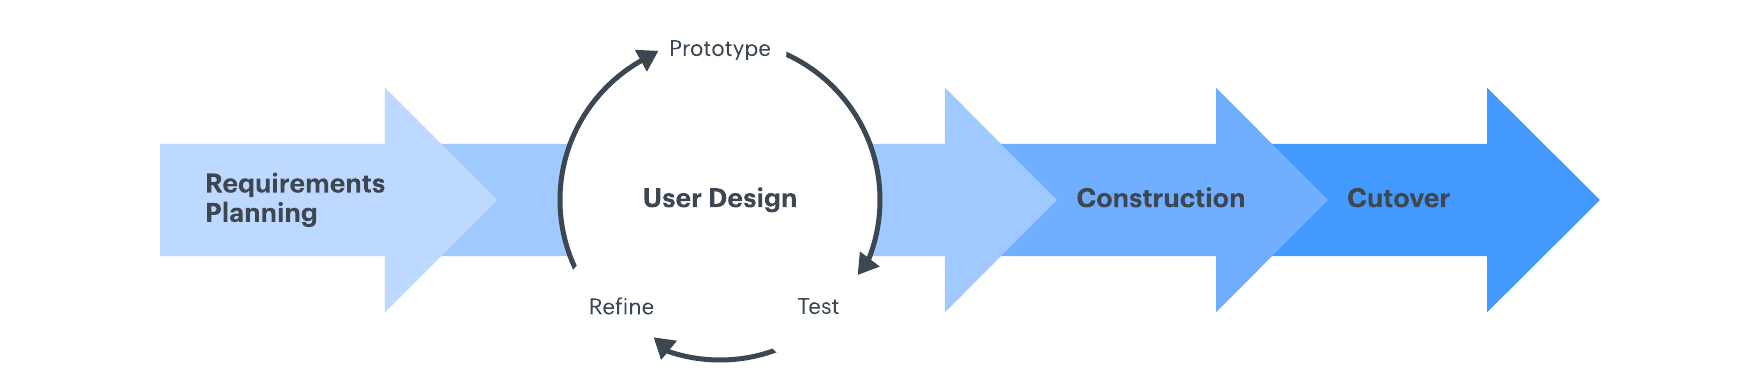
\includegraphics[scale=0.7]{RAD}
\end{center}
\begin{itemize}
	\item Allows for greater flexibility than waterfall, but not as much as agile
\end{itemize}


\section{Spiral}

\begin{center}
	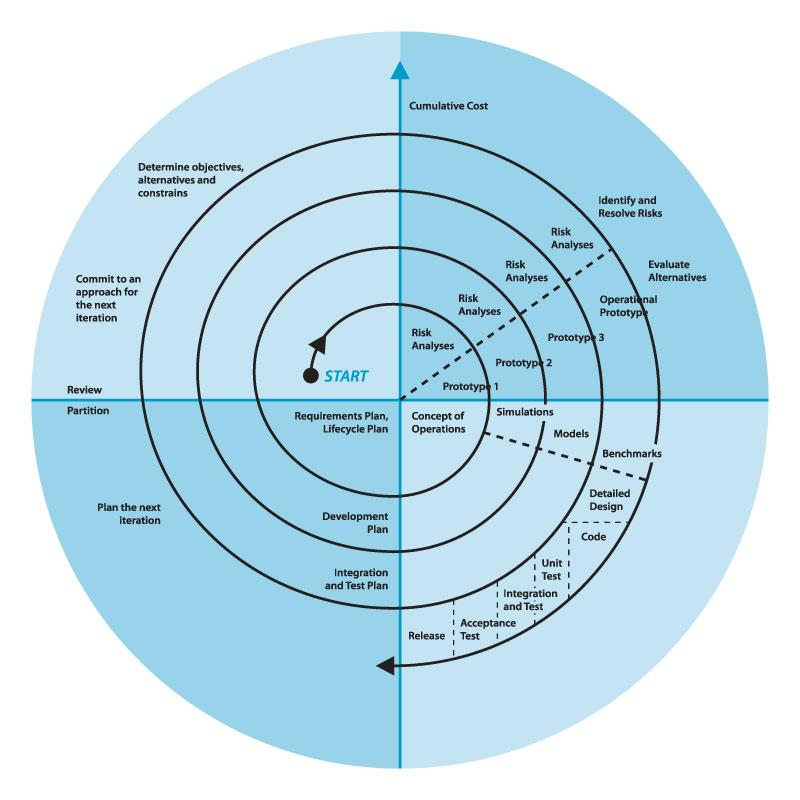
\includegraphics[scale=0.7]{Spiral}
\end{center}
\begin{itemize}
	\item Linear model
	\item Risk analysis - Make sure you are able to complete the part of the spiral before the next analysis 
\end{itemize}
\section{Prototyping}
\begin{center}
	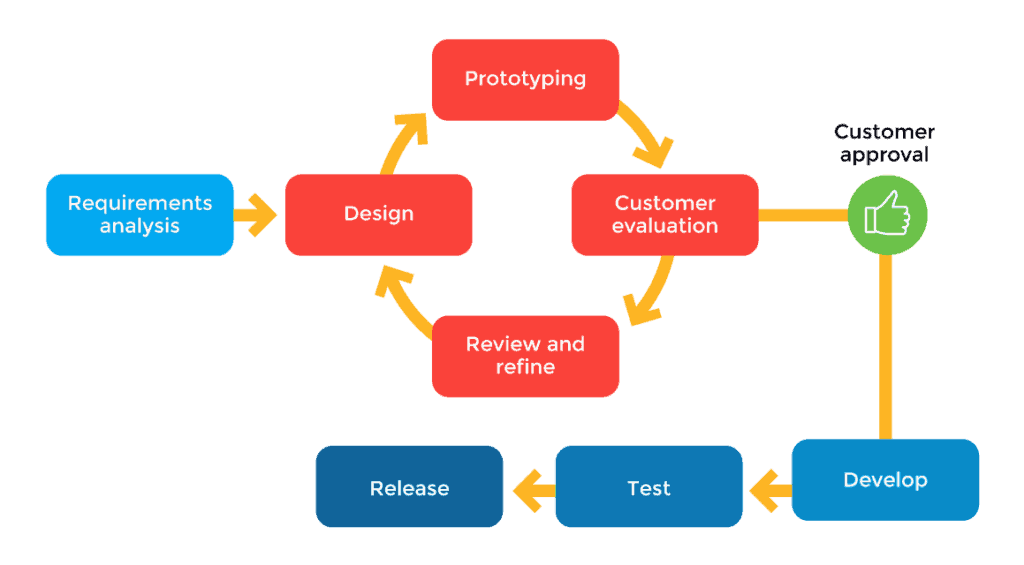
\includegraphics[scale=0.7]{Prototyping}
\end{center}
\section{Lean Innovation}
\begin{center}
	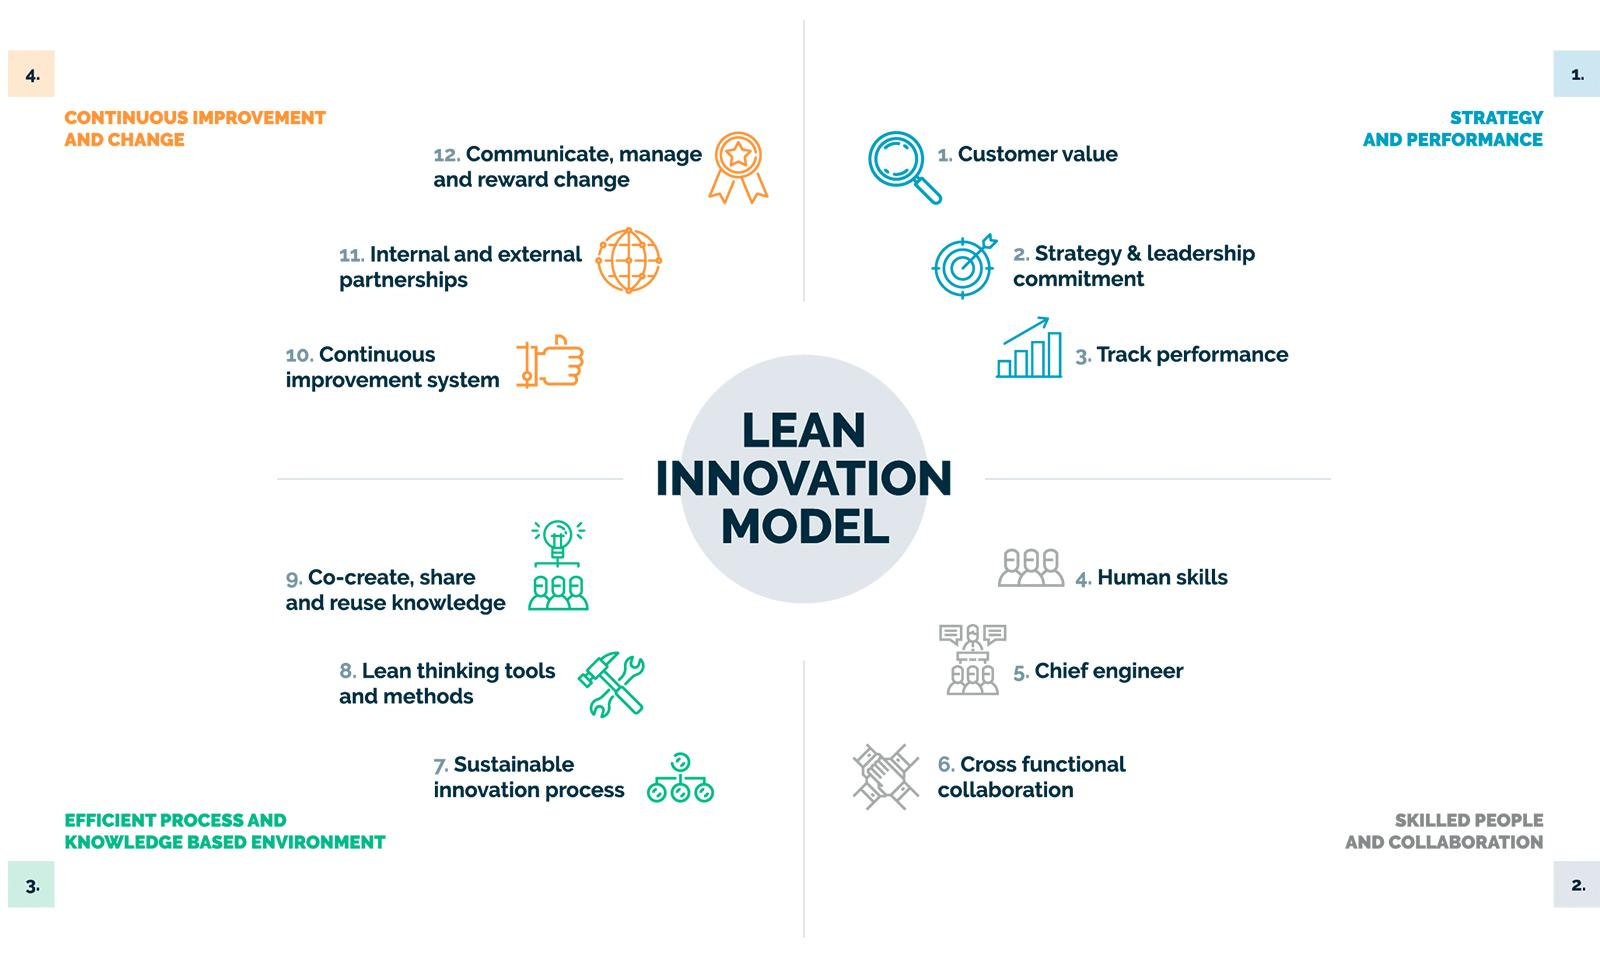
\includegraphics[scale=0.4]{Lean-Innovation}
\end{center}
\begin{center}
	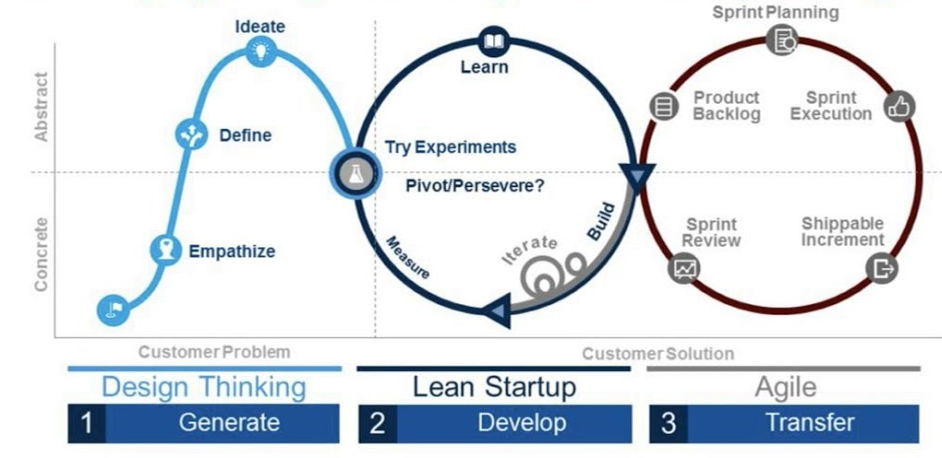
\includegraphics[scale=0.7]{Lean}
\end{center}
\section{DevOps}
\begin{center}
	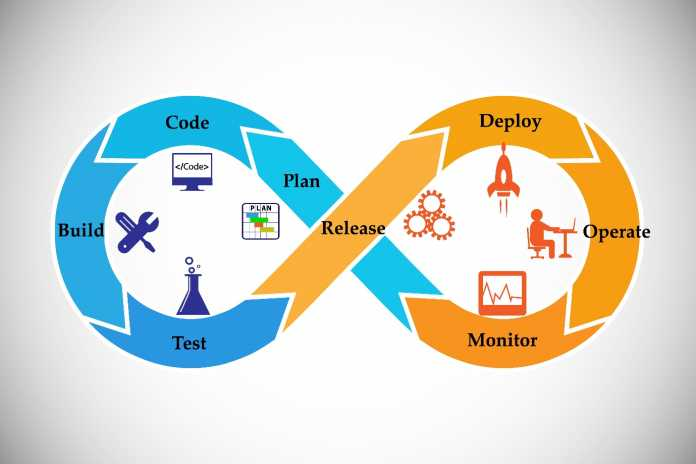
\includegraphics[scale=0.7]{DevOps}
\end{center}
\begin{center}
	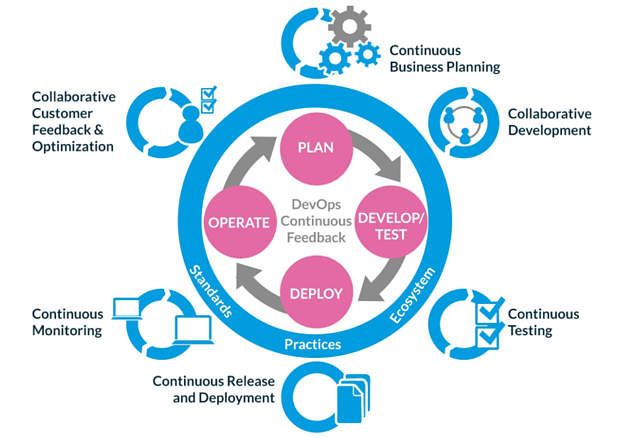
\includegraphics[scale=0.7]{DevOps1}
\end{center}
\section{Not a Software Development Model}
\begin{itemize}
	\item ITIL (Information Technology Infrastructure Library) v4
	\item Linked to DevOps, Agile and Lean
	\item Service - Providing benefit to a person
	\item Value - Return on what you are putting in
\end{itemize}
\begin{center}
	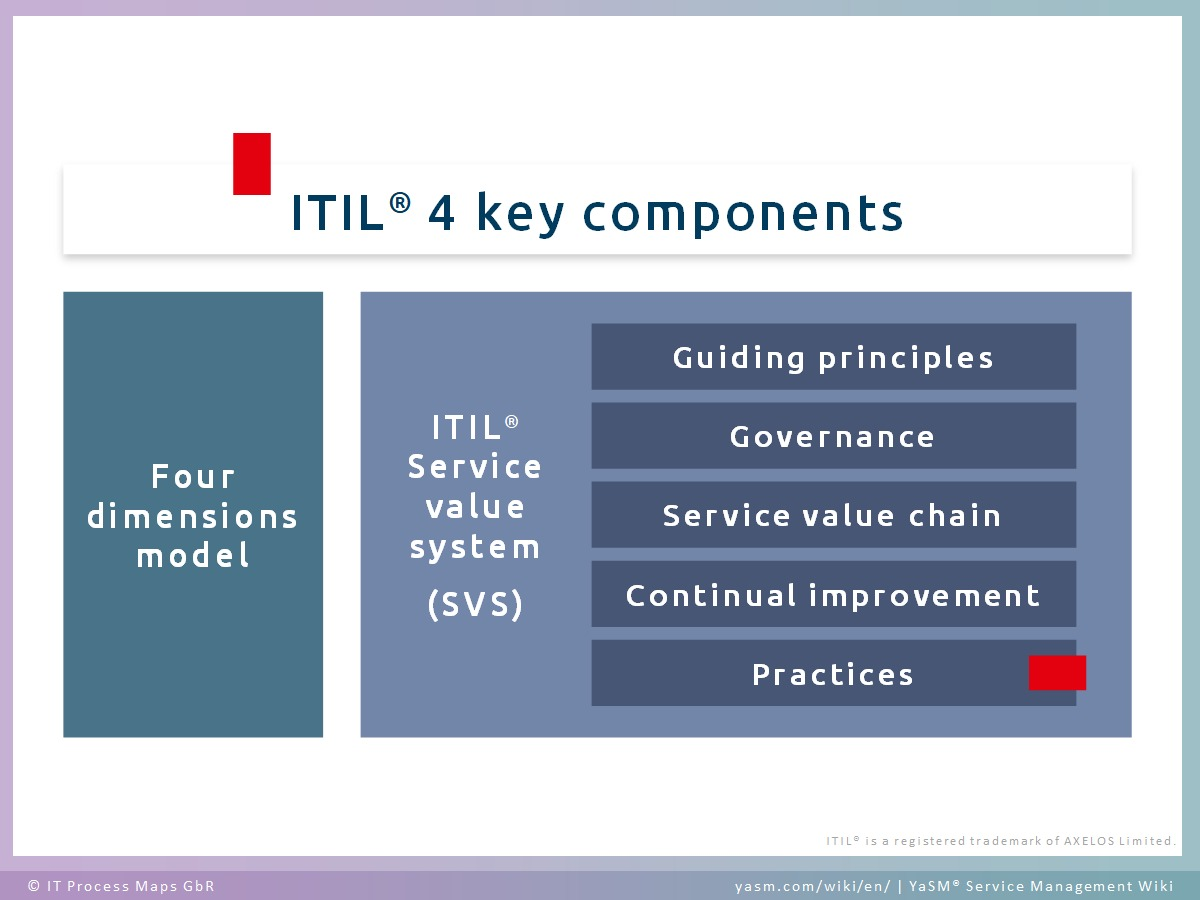
\includegraphics[scale=0.7]{ITIL}
\end{center}



\end{document}